\chapter{Programming concepts for data analysis}

This chapter introduces readers to the basics of programming. It
outlines how to install the software (R and Python) used in this book,
explains how to deal with objects, statements, expressions, variables
and different types of data, and shows how to create and understand
simple control structures such as loops and conditions.

\section{Installing R and Python}
\label{sec:installing}

In the previous chapter, we had fun with data using the provided
docker, which meant that there were very few things to install in
order to run the initial examples. However, if you want to enjoy all
the power of computational analysis of communication you must be able
to install from scratch all the necessary software, packages and
dependencies in order to complete your first steps as a programmer and
then be able to write, adapt and run code. Nowadays you may find many
online and cloud services that provide web interfaces to run code,
both in R and Python, which might result useful depending on your
needs. Nevertheless, we encourage you to install on your local
computer all the basic software and packages that we will use
throughout this book and that you will likely use in the near future
in order to apply the learned techniques in your own research.

As we already justified in the introduction of this book, R and Python
are the most popular programming languages that data scientists and
computational scholars have adopted to conduct their work.  Now, we
should download and install these open-source and free applications on
our local computers and become familiar with some additional
resources, such as popular \emph{integrated development environment}
(IDEs) and notebooks, which provide a more friendly interaction with
your code. All the resources are typically available for MacOS,
Windows and Linux, but keep in mind that their implementation in each
operating system might differ (for example, in the way you install the
software or when writing the absolute or relative paths in the code).


\subsection{Installing R}

Firstly, we will install R and its most popular IDE RStudio, and we
will learn how to install additional packages and how to run a
script. R is an object-based programming language
orientated to statistical computing that can be used for most of the
stages of computational analysis of communication.  If you are
completely new to R, but familiar with other popular
statistical packages in social sciences (such as SPSS or STATA), you
will find that you can perform in R many already-known statistical
operations. If you are not familiar with other statistical packages,
do not panic, we will guide you from the very beginning. Unlike
many traditional software that requires just one complete and initial
installation, when working with R, we will first install the raw
programming language and then we will keep on installing additional
components during all of our journey. It might sound cumbersome, but
in fact it will make your work more powerful and flexible, since you
will be able to choose the best way to interact with R and especially
you will select the packages that are suitable for your project.

Now, let's install R. You can go the official R
webpage\footnote{https://www.r-project.org}, where you will find lots
of valuable information about the environment as well as the necessary
documentation for working in R.  There are different versions of R,
since there is a global community of developers that help to improve
the software continously. You should go the CRAN mirrors and click onto
any mirror (or the one you consider more close to your place of
work). Within the mirror you can download the version you need
depending of your operating system (figure~\ref{fig:cran}). In case
you're not familiar with terms ``CRAN'' or ``mirror'', the first
refers to the \textit{Comprehensive R Archive Network}, which is an
online repository of R packages; and the second, to the server where a
copy of any package is available for download.

\note{If you use Linux, you may want to install R via your package
  manager (such as \texttt{apt} on Debian and Ubuntu) instead.}


\begin{figure}
\centering
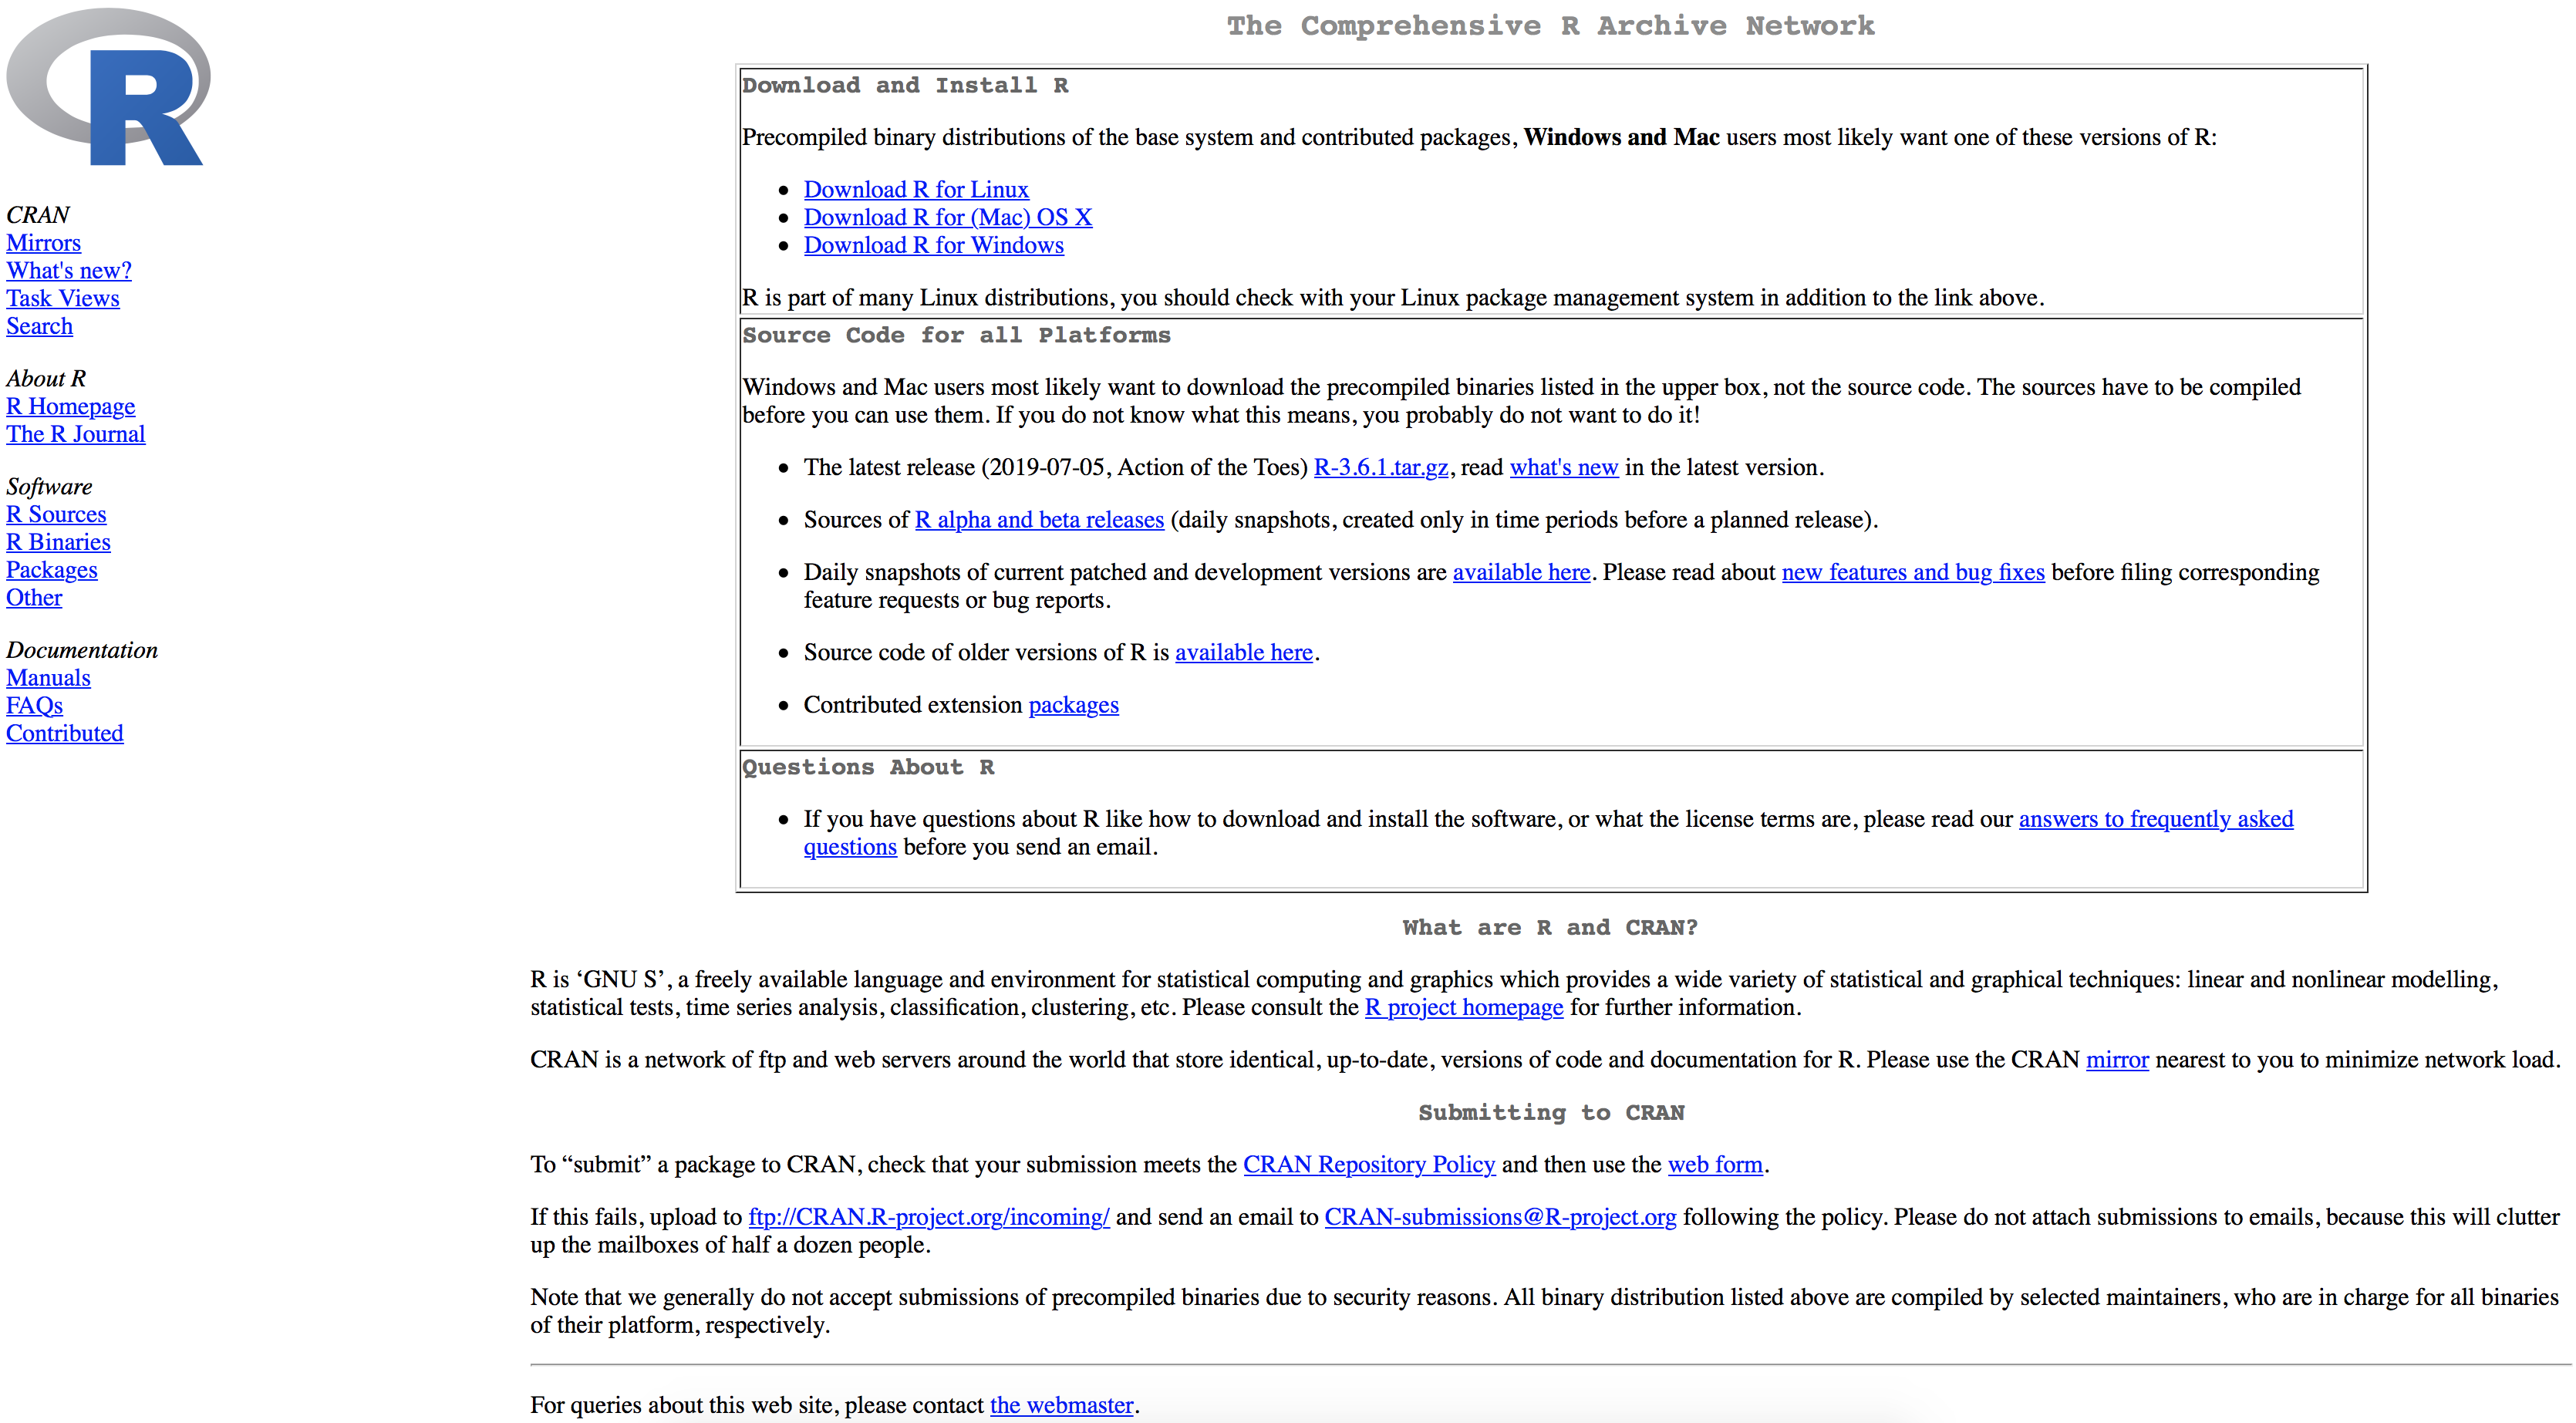
\includegraphics[width=0.9\linewidth]{figures/ch3_cran}
\caption{The Comprehensive R Archive Network.}
\label{fig:cran}
\end{figure}

Once you have downloaded and installed R on your computer (follow the
instructions on the page for each operating system), you will be able
to open an R console (figure~\ref{fig:r_console}), where you can
perform all operations, from reading datasets to execute sophisticated
data analysis. If you are new to computer science jargon, it is worthy
to clarify what a \textit{console} is and what is the difference with
a \textit{script}. In a console, you can write and execute commands
line-by-line. In fact, all computers and operating systems have
terminals or consoles, which help us to interact with the machine,
from listing files of a given folder (e.g. command \texttt{ls} on
Linux and MacOS) to install software, apps or utilities. The point is
that any console is an active tool that normally executes the line or
group of lines after you press the \textit{enter} button.
If, instead of typing each command line-by-line into your console,
you put several of such command lines into a text document, we call it a \textit{script}.

If you want to execute some more complex set of code lines, you may
wish to write and test them in a separate file (the script) that you
can save and also run from the console. This distinction is very
useful in R, as you will normally work with both, an R script file and
an R console, in order to run your computation.

\begin{figure}
\centering
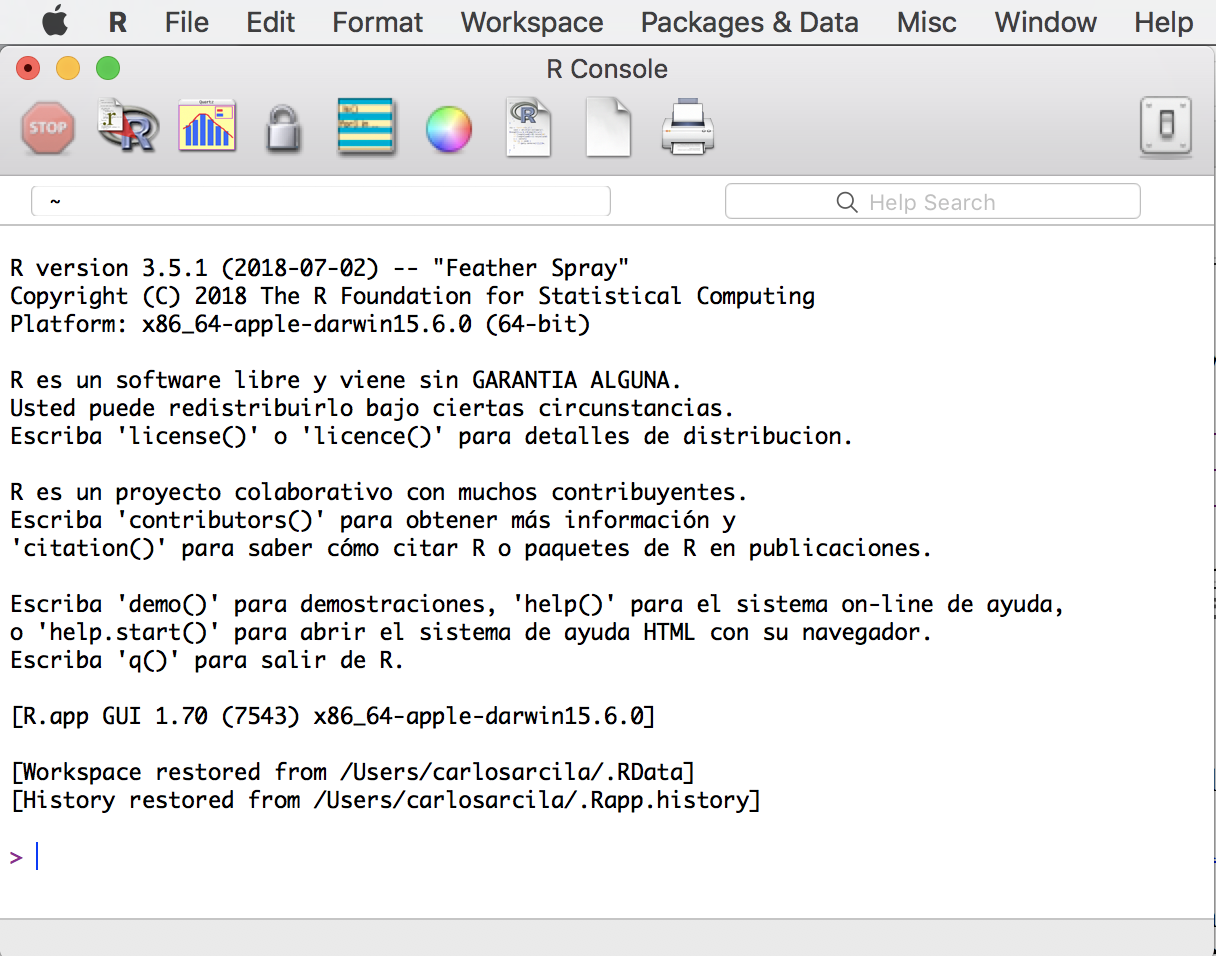
\includegraphics[width=0.9\linewidth]{figures/ch3_r_console}
\caption{R Console.}
\label{fig:r_console}
\end{figure}

\newcommand*{\icon}{
\includegraphics[scale=0.8]{figures/document_icon}}%
\newcommand*{\doc}{
\includegraphics[scale=0.7]{figures/r_document_icon}}%
\newcommand*{\rcom}{
\includegraphics[scale=0.8]{figures/r_icon}}%

In the R Console you will just have an empty line beginning with the
sign \textgreater, where you can write any command, and also a menu
with some useful icons. For example, the empty document icon \icon
\ will allow you to create a new R document and write there your
code. You can later use R document icon \doc \ to modify any given
script or the general R icon \rcom \ to run the script or to load data
in R. On the upper menu you will also find convenient tools such as
Workspace or Packages \& Data. Because R is an
object-orientated programming language, which means that all
operations are performed with objects that we create or import, from
simple variables to complex recursive functions. If you create an
object \texttt{x} with the value 17 (x \textless- 17), this object will
be loaded into RAM memory so you can access by just typing \texttt{x}.
The menu Workspace will let you know which objects
have been uploaded to this virtual space. We will go back to this
issue later in this chapter when we discuss statements, expressions,
variables, functions and methods. R can perform many statistical operations with its
raw language, but one of its greatest advantages is that we can use
existing packages (also called libraries) that others have created to
simplify our coding and to expand our possibilities in data
analysis. You can find these packages in the CRAN, ensuring that there
has been a minimum set of verification steps for that code, or
directly from a developer webpage or repository. The menu Packages \&
Data will help you to manage and install packages, as well as to load
pre-existing data (freely available datasets we can work with).

If you are unfamiliar with dealing with datasets in a coding
environment, probably the first package you will be willing to install
is \pkg{R Commander}\footnote{https://cran.r-project.org/web/packages/Rcmdr/index.html},
or \pkg{Rcmdr} for short, which is a graphical user interface for R that
helps you to interact with data in a more visual way, similar to SPSS.
You can install this package either by using the R Package Installer
tool (Menu \textgreater Packages \& Data \textgreater Package
Installer), or by typing the next syntax on your R Console:

\codex{chapter03/installpackages.r}

Be patient, it will take some time to download and install on your
local computer all the files and dependencies necessary to run \pkg{R
  Commander}. The good thing is that you have run your first line of
code and you will notice that it is not that difficult; most of the
commands you will use will follow a similar logic. In this case you
have a native command (install) with a module (packages) and an
argument (``Rcmdr'') with an option (dependencies=TRUE). It is worth
mentioning that once you have installed any package on your computer,
you have to import it it in the R environment every time you are going
to work with it. This means that you have to indicate either on your R
console or R Document, which libraries you will be using, so the
program can load the package. The are two common methods to load or
attach an add-on package: \fn{require} and \fn{library}. \fn{require}
will return an error if the package is not installed. Whenever you
want to know more about a method you can call for documentation using
the |?| symbol, e.g. |?require|.

Now, let’s load R Commander by typing |require(Rcmdr)| into the R consule.

In this case, by loading \pkg{Rcmdr} a pop-up window will be displayed
with the graphical interface to work with data and run basic
statistics. In most other cases, no window will show up, but the
package will be loaded in the backend so you can use all its
functions. For example, if we are working a on an R script (.r or .R)
where we write a set of instructions that need any particular package
we should call that package in the file before it performs any
operation included in it (by just entering a line such as
|library(<the_package>)|.

With this line you ensure that you will not get an error message
warning you that certain function does not exist or has not been
properly called when your are running the script.

Now that you have learned how to install R and its packages on your
computer, we should move on to get familiar with additional resources
that are of great help when working with R. In particular we introduce
RStudio, which is an IDE (Integrated Development Environment),
free of charge and open source that will
make our computational journey with R much more friendly and
easier. Among many other advantages, in this environment you will have
a workspace where you can simultaneously visualize your R documents
(.r files), the R console, the objects or variables you load to memory
and files or packages you are dealing with. You can find a desktop
application that will run locally on your computer (RStudio Desktop)
or a web-server version that you can install on a remote server and
run from any web browser via Internet (RStudio Server). If it is your
first time on this environment, we encourage you to download and
install RStudio Desktop (figure~\ref{fig:r_studio}) from its official
website\footnote{https://www.rstudio.com/products/rstudio/download/}. As
in the case of R, choose the appropriate installation file for
your operating system (MacOS, Windows, Linux) and get the latest
version.

\begin{figure}
\centering
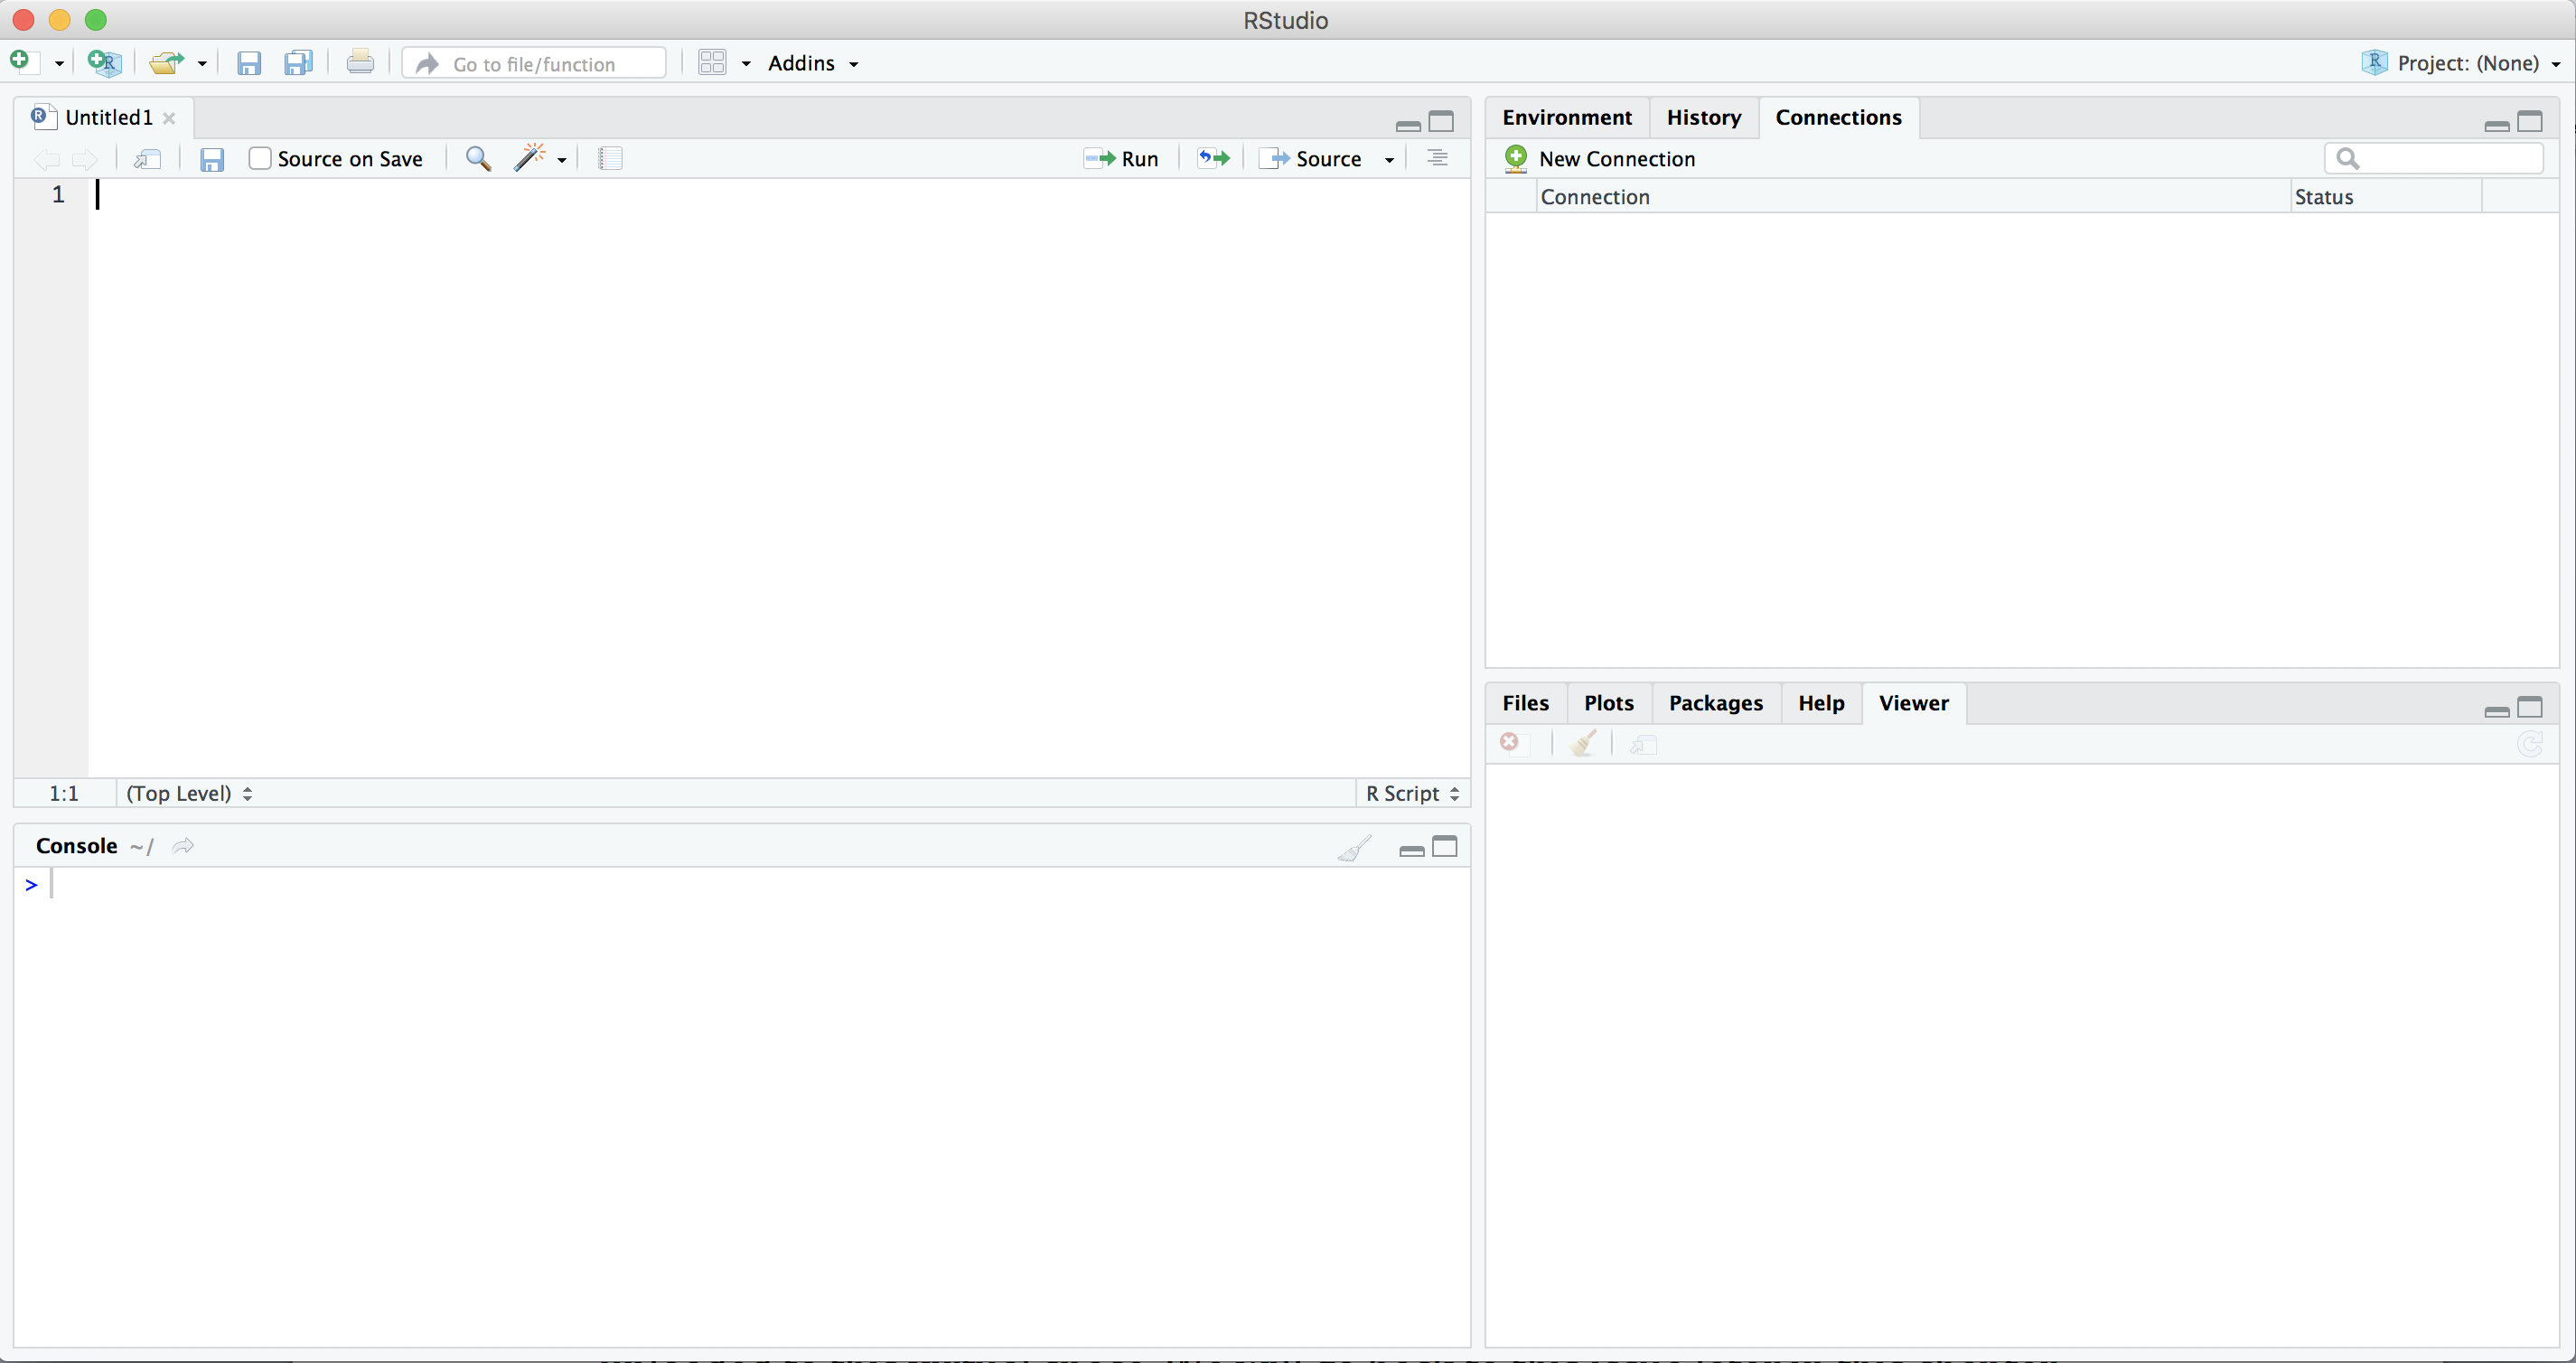
\includegraphics[width=0.9\linewidth]{figures/ch3_r_studio}
\caption{RStudio Desktop}
\label{fig:r_studio}
\end{figure}

In RStudio you will see by default four main integrated windows (you
may later reconfigure it), and the upper menu. In the up-left window,
you can visualize and edit all the files you will work with, in
special R documents (|.r|), data, and R Markdown documents (|.rmd|).
If it is the first time you hear about Markdown, keep this format in
mind because it is a markup language for plain text that will help you
to work with reproducible R documents based on a very simple syntax
and ready-to-export to most universal formats such as HTML or PDF. The
down-left window is the R console where you can directly write a
syntax or where your will get the outcome from the code you have
written and run in the R document. Look at the up-left window
and notice that there is a button named \emph{run}, which you will
often use. By selecting partial or total lines of code in your script
and clicking on this button you will execute the code and get the
results in the console.  As you will realize with the first practices,
it will be very useful to have the script in one window and gradually
run parts of the code, instead of executing the whole document at once
or to run it line by line in the console.

In the right side of RStudio workspace you will find two additional
windows. In the up-right window there are three tabs. You will mostly
use \emph{environment} and \emph{history}, and seldom
\emph{connection} (just to connect to existing data sources such as
those from ODBC or Spark). In \emph{environment} you can manage your
workspace (the set of elements you need to deploy for data analysis)
and have a list of the objects you have uploaded to it. You may also
import datasets with this tool, and most importantly, you can save
your workspace or open a previous one. In \emph{history} you will
have an inventory of code executions, which you can save to a file, or
move directly to console or to an R document. In the down-right window
you will have five more useful tabs. In \emph{files} you can explore
your computer and manage all the files you may use for the project,
including importing datasets. In \emph{plots}, \emph{help} and
\emph{viewer}, you can visualize the outputs figures, documentation
and general outcomes, respectively, that you have executed in your
script. Finally, the tab for \emph{packages} will be of great
utility since it will let you install or update packages from CRAN or
even from a file saved on your computer with a friendly interface.


\subsection{Installing Python}

Now that you have installed R and RStudio, let's change to Python. As
many computational scientists do, we will jump from one application to
another throughout this book, so do not worry if you have to wear two
hats the same day, even at the very same time! The first thing will be
to install Python on your local computer (though some operating
systems come already with it as a default). As explained in \refchap{introduction}, Python is an object-orientated programming language
and it is probably the favourite language of computational and data
scientists in all disciplines around the world. There are different
releases of Python, but you will usually find a distinction between
versions of Python 2 and those of Python 3, since some syntax and
functions change from one to another. In this book, we will explain
Python 3.x and all our examples and exercises will be written for this
version. Notice that you might install different versions of Python on
your local computer, and also create specific virtual environments
(including a Python version and all its libraries and dependencies).
By doing this, you will be able to run any version depending on your
needs. Thus, if you do not have already Python on your
computer \footnote{There are different ways to check if you already
  have it. For example, if you are in MacOS, you can open your system
  terminal and type \texttt{python -V} or \texttt{python --version}, and
  you will get a message with the version that is working by default
  in your computer or that has been set as an environment
  variable. There might be different versions already installed, so
  you might check directly for them: \texttt{python2 --version} or
  \texttt{python3 --version}.}, the first thing will be to download it
and install it from its official
webpage\footnote{https://www.python.org/downloads/}, selecting the
right software according to your operating system (Windows,
Linux/UNIX, Mac OS X).

\note{If you use Linux, you may want to install Python via your package
  manager (such as \texttt{apt} on Debian and Ubuntu) instead.}


During the installation, you will be informed that some additional
features will be installed along with Python: normally an
\emph{integrated development environment} called \pkg{IDLE}, a package
manager called \pkg{pip} and \emph{documentation}. Even though more
advanced IDEs are available (for instance, you may like \pkg{spyder},
which looks a lot like \pkg{Rstudio}, or \pkg{pycharm}, which has a lot of functionality that appeal to advanced programmers), IDLE will
provide you with a basic interface to work with Python files (|.py|)
and the Python console. \pkg{pip} is a basic package that will help
you to install and manage more software packages within Python. And
documentation will provide you with basic help to work in this
programming language.  In addition, you might be asked if you
want to add Python to your path, which means that you set the
\emph{path variable} in order to call the executable software from
your \emph{system terminal} just by typing the word |python|. We
recommend selecting this option.  If you have never worked before with
the system terminal of your computer, probably this is a good
opportunity to know what and where it is. With this terminal you can
interact with your machine and navigate through your files, create new
ones, install programs, execute scripts, etc.  Everything you already
do in your friendly and graphic interface in Windows, MacOS or Linux,
but performing it only with commands and code. Well, if you already
downloaded and installed Python, you may open your system
terminal\footnote{The terminal will look slightly different depending
  on your operating system. In MacOS or Linux you can find it the
  `Terminal' in the Utilities folder in Applications; and in Windows
  you can get the `Command Prompt' in the Accessories folder in the
  All Programs menu.}  and launch Python from it! First, type
|python --V| and press enter to check your current installed version and then
just type |python| and you will open the software from the very same
system terminal.

\begin{figure}
\centering
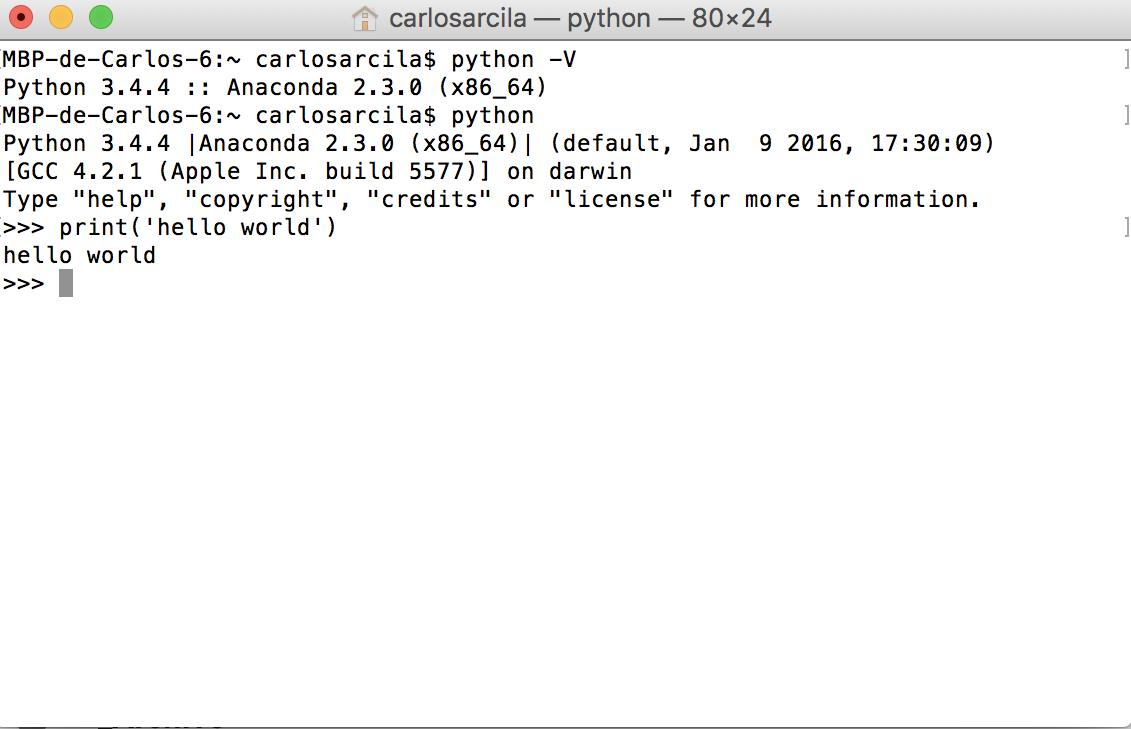
\includegraphics[width=0.9\linewidth]{figures/ch3_python_from_terminal}
\caption{Python launched from the Terminal.}
\label{fig:python_from_terminal}
\end{figure}

So, welcome to Python. You are now in the Python console, from where
you freely operate this programming language. As it is a console,
every line of code you type will be executed by pushing enter onto
your keyboard, which means that if you have complex code you will
mostly prefer to write the script in a Python file (.py) or similar
(i.e. a notebook) and then run this file. However, as a first exercise
it will be worth to keep the Python console open and write your first
line of code on it, using the native function \fn{print} (see \refex{helloworld}).

\codex{chapter03/helloworld.py}

After running this line, you will get your first result or
output (Figure~\ref{fig:python_from_terminal}), which will be to
display on the screen a sequence of characters, called a
\emph{string}. You might tell your colleagues that you have written
your first computer program, just as many computer scientists have
done so in their first programming class. We will come back to coding
in Python in the next sections. Now, let’s try to install some
packages. Remember, that similar to R, in Python we can build every
function from scratch, but there are many libraries or packages that
will make our life easier, and some times, even more fun. There are
different ways of installing a new package in Python, but the most
classical one is by using the command pip from your system
terminal. In order to quit the Python console and return to the system
terminal, just type |exit()| and press Enter.

Once you are back in your system terminal again you can use pip to
install any package under your default python version (notice that if
you have different versions or environments of Python, the package
will not be installed in all of them).  In the last versions of Python
some packages such as \pkg{numpy} (for computing large
multi-dimensional arrays and matrices) will be included by default,
but most likely you will need to install many others.  This is the
case of \pkg{tweepy}, which is a library to connect to the API's of
Twitter and we will work with it in chapter [SCRAPING ONLINE DATA]. To
install this package just run the next line on your system terminal:

|pip install tweepy|

With this simple command, you will download and install this powerful
package on your computer. You may try to check if you can now use the
package, just by going again to Python console and use the command
import to bring the library to your current session.

\codex[caption=Importing a python module]{chapter03/importtweepy.py}

If no error is shown, you can be happy that you successfully
installed your first package in Python in just few seconds, using the
system terminal and the raw Python software. Far beyond this basic
environment, you might find more functionalities and shortcuts in this
programming language if you use additional resources, such as any IDE
or notebook, which will help you to interact with Python. In this
book, we will mention three IDEs (IDLE, PyCharm and Spyder) and one
notebook (Jupyter Notebook). IDLE (\emph{integrated development
  learning environment}) is a specific IDE provided for Python and
which you might have already installed when you downloaded
Python. IDLE has a Python console (\emph{shell}) where you can directly
write and execute code, and will also allow you to create Python files
(|.py|) in a document-like window with some basic functionalities at the
time of writing, such a colouring the code (depending on their
function in the script), easy indentation or code debugging
(figure~\ref{fig:python_idle}).  This will make your journey easier
and more productive.

\begin{figure}
\centering
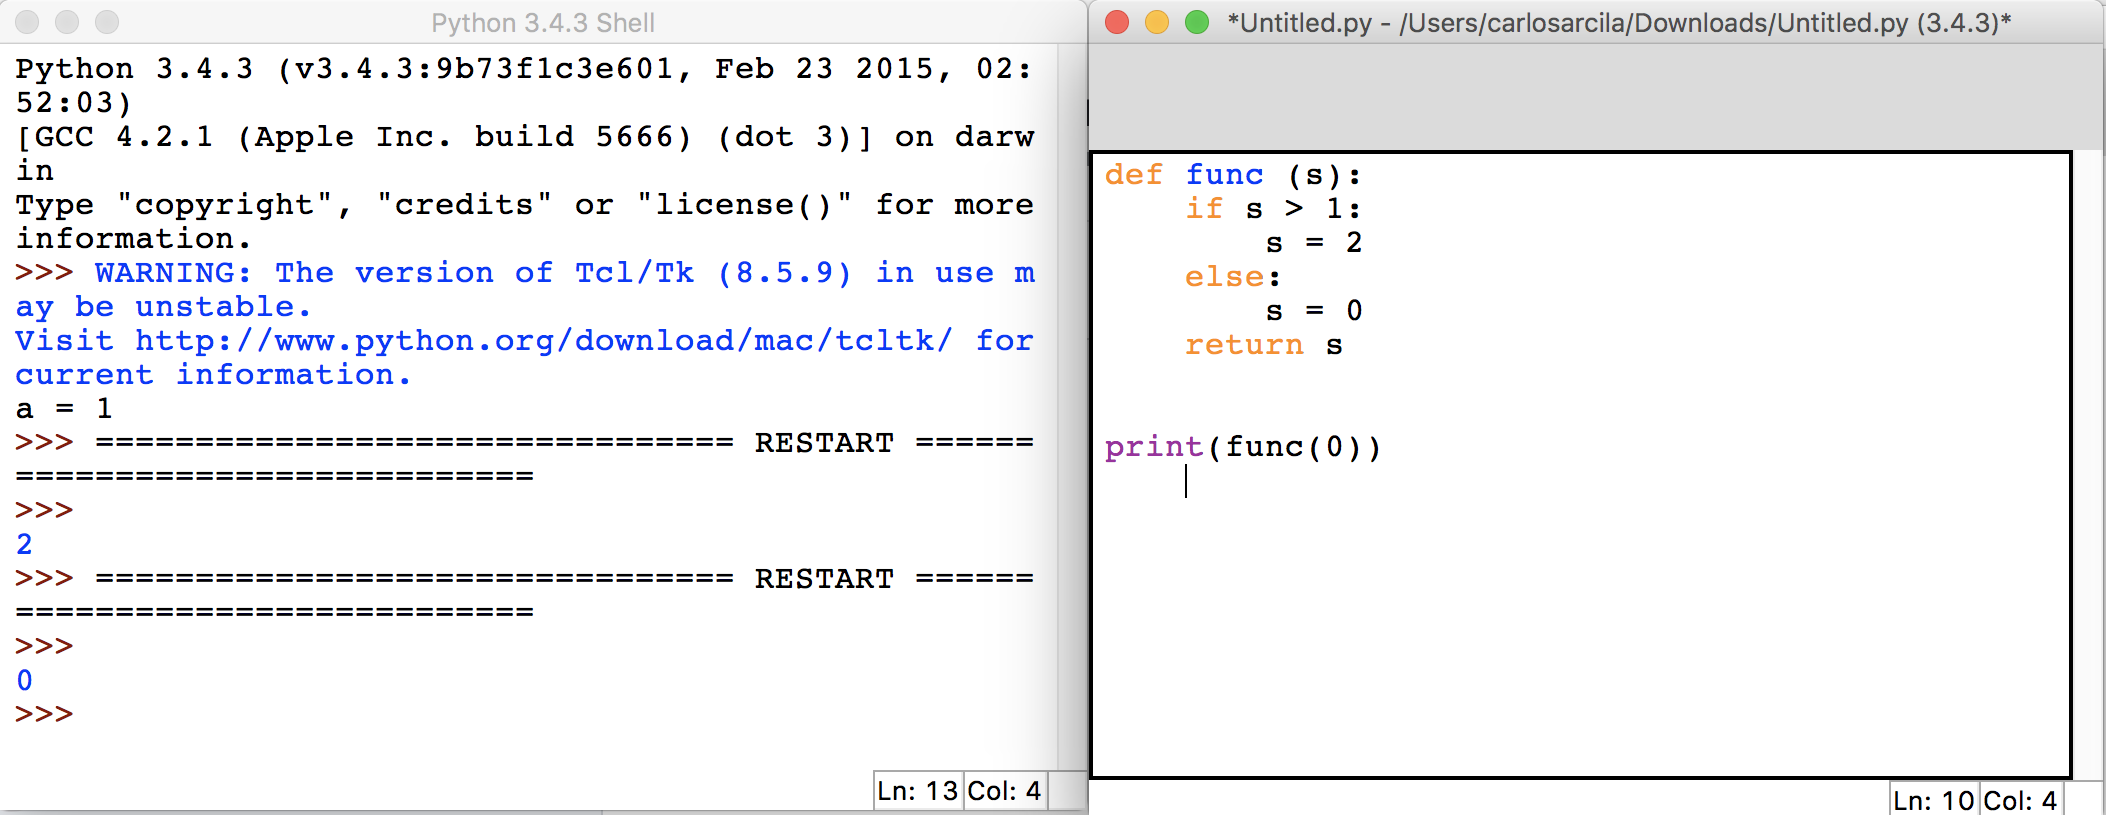
\includegraphics[width=0.9\linewidth]{figures/ch3_python_idle}
\caption{Python shell (left) and file (right) in IDLE.}
\label{fig:python_idle}
\end{figure}

The next useful IDE is \pkg{PyCharm}, which provides an even more graphical
and integrated interface to deal with Python.  Developed by JetBrains,
PyCharm has a free and open source \emph{Community} version that you
can download and install on your local computer from its
webpage\footnote{https://www.jetbrains.com/pycharm/download/} with
options for Windows, MacOS and Linux. Once installed you can connect
the software to any of the already installed versions of Python or
even easily create \emph{virtual environments} to work on your
projects. These virtual environments are isolated Python environments
that will let you have a specific configuration and dependencies to
work with in a project. For example, you may create one with an older
version of Python, including specific releases of libraries.  You can
equally achieve this with the pip command from your system terminal:
|pip install virtualenv|.
 
But PyCharm will help you to manage it with a graphical and friendly
interface. The same happens with installing packages: using the
\emph{Project} sub-menu from the \emph{Preferences} menu, you can
install, update and delete any package related to any version of
Python or virtual environment. In fact, easily dealing with Python
versions and libraries is one of the main reasons why we recommend to
new \emph{pythoners} to use PyCharm. But there are even more
advantages.

Just like RStudio, PyCharm is an integrated interface that shows us
different adjustable windows with a unique frame that we create for
every project we open. Every time you create a project you have to
name it, save it to a specific location (a folder where all your files
will be stored) and choose an interpreter (a Python version or
environment used by default in the project). Once created, you can
begin to work on it with three main windows or sub-frames
(Figure~\ref{fig:pycharm}). The upper-left window contains the project
structure and files. You can easily create or import folders and files
and then navigate through them in this area. For example, by clicking
on the right button of your mouse (or by going to File \textgreater
New) you can create a new Python file (i.e. my\_first\_script.py) and
organize your scripts by folders. In the upper-right window you will
be able to visualize and modify the editable files contained in a
project. All the open files will be in this window and you can access
to any of them by clicking on its name situated in the upper tabs. In
the low window you will find the output space as well as the Python
and system consoles. This separation is very useful since you can work
on your .py script (also with colour, indentation and error detection
facilities), run it (from the \emph{Run} Menu) and produce the
expected output in a separate window within the same frame.

\begin{figure}
\centering
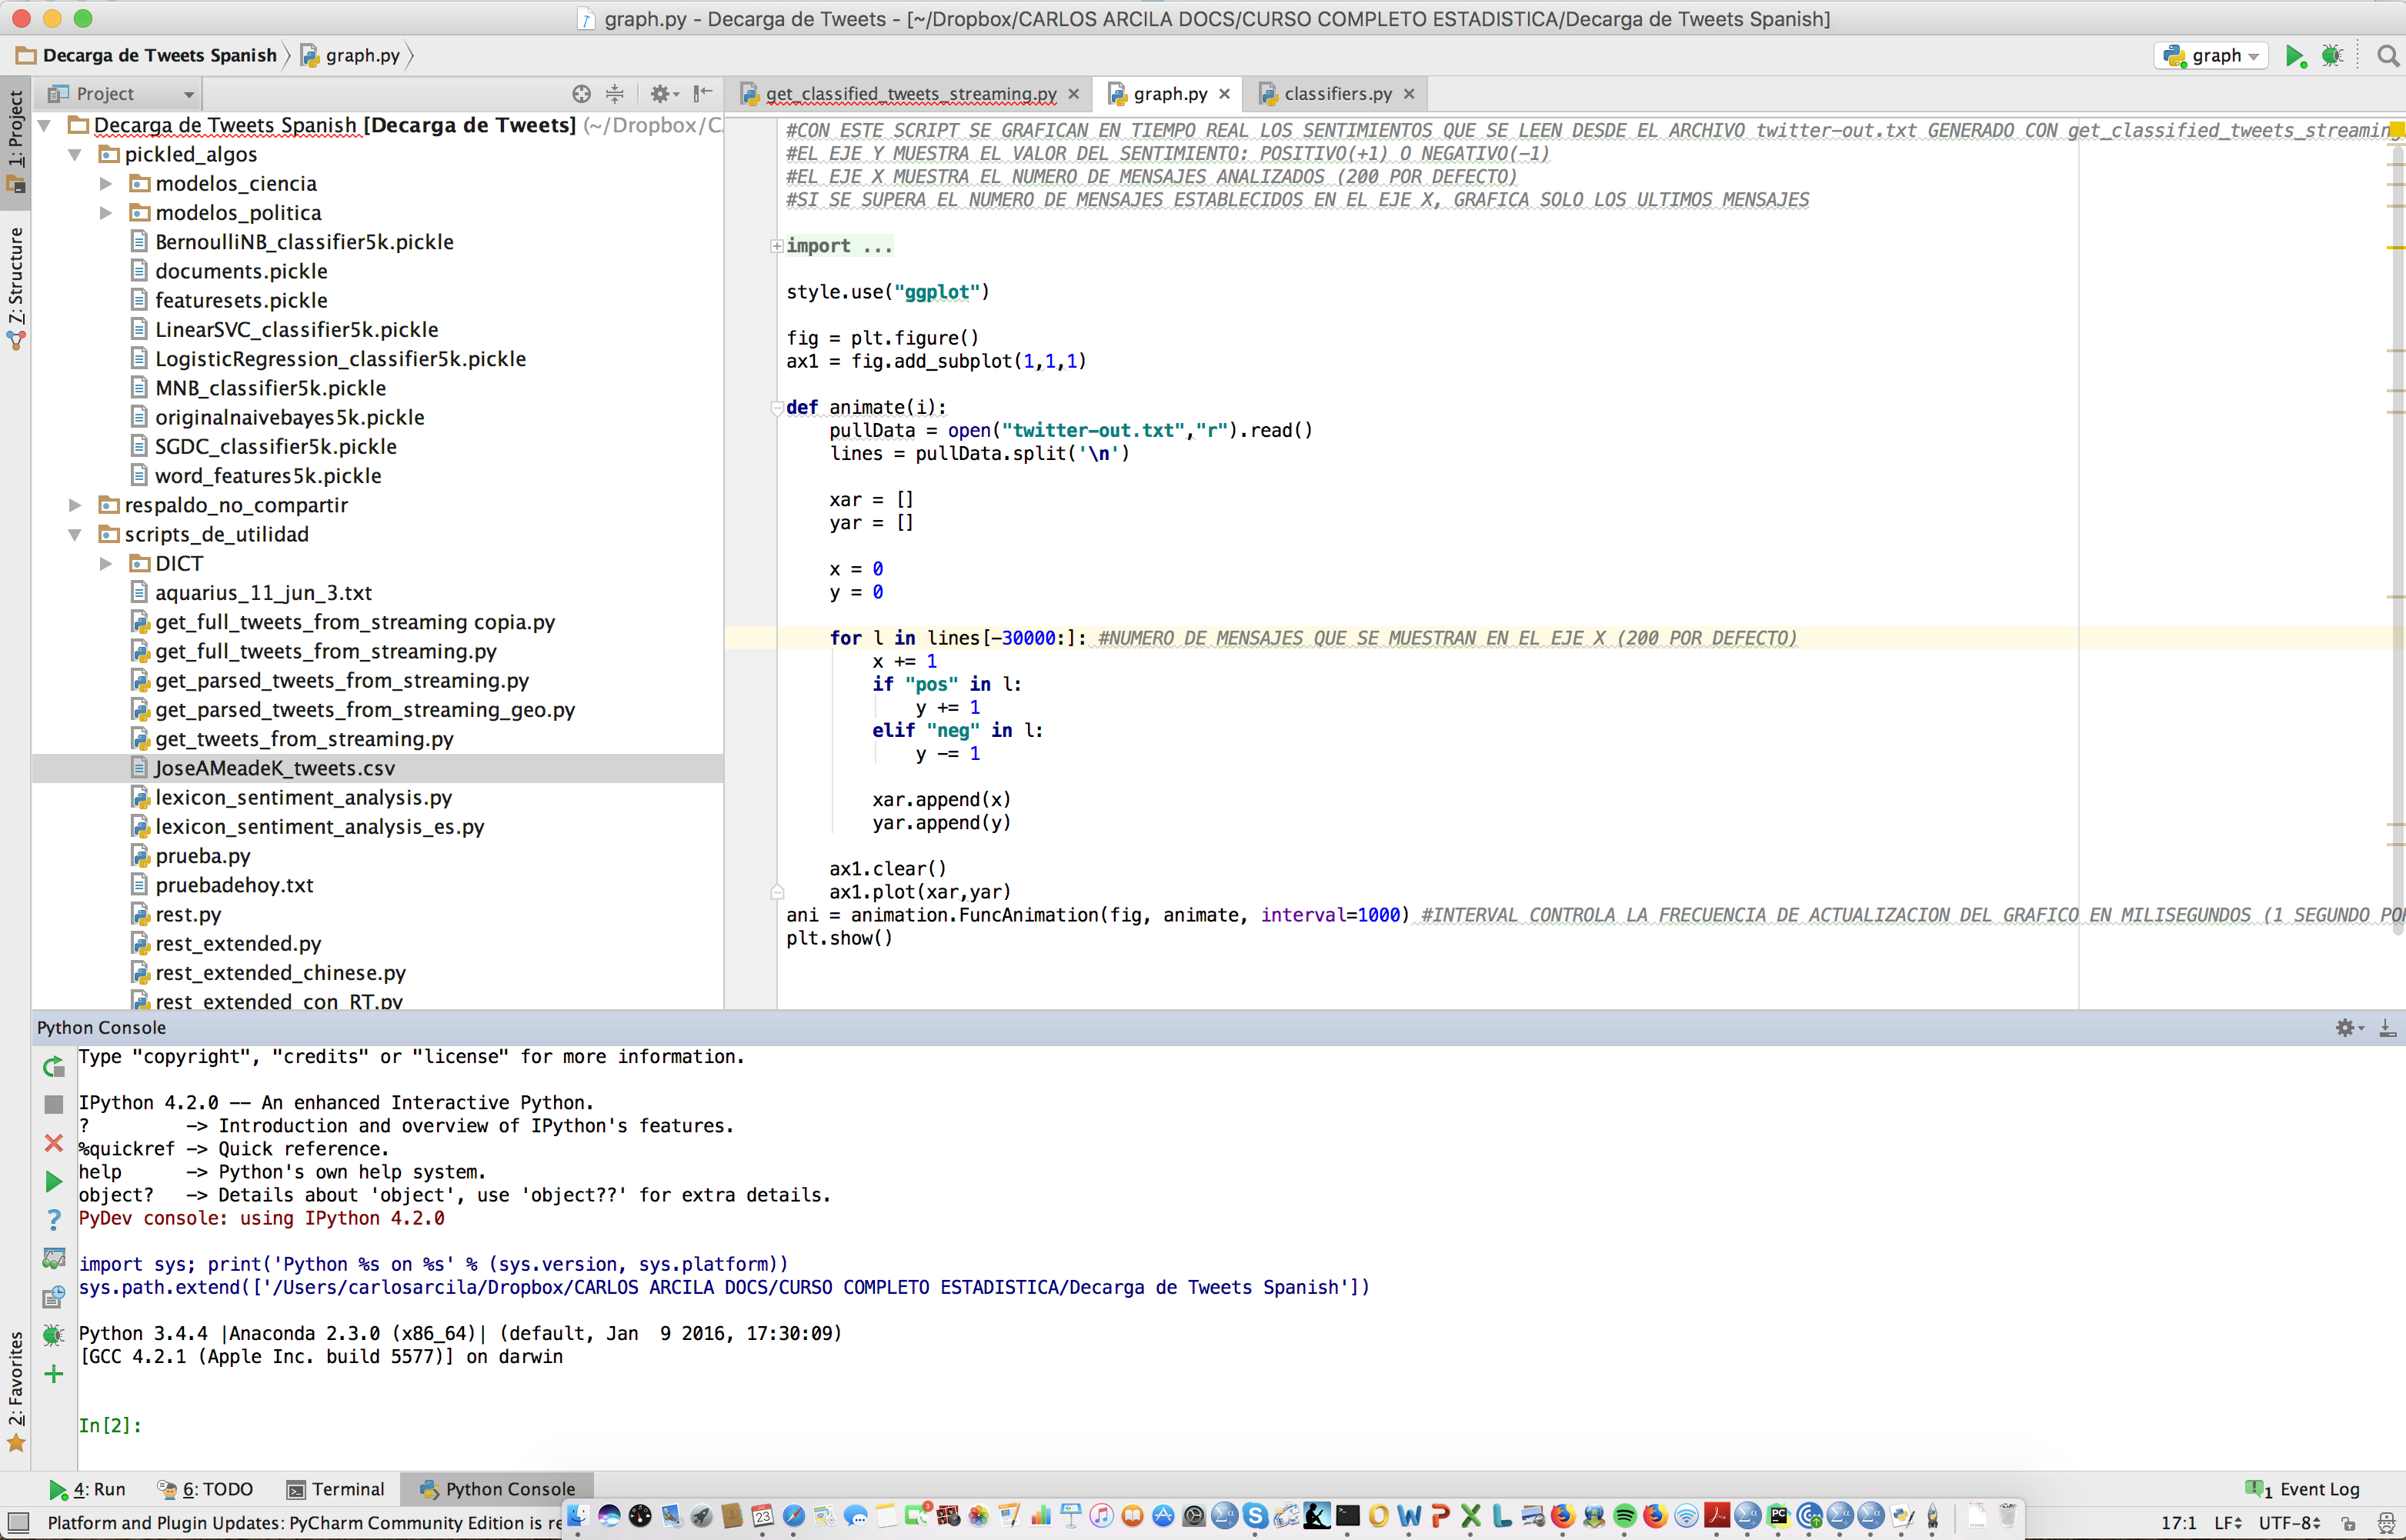
\includegraphics[width=0.9\linewidth]{figures/ch3_pycharm}
\caption{PyCharm environment.}
\label{fig:pycharm}
\end{figure}

The next two extra tools we would like you to familiarize with are
Spyder and Jupyter Notebook. Spyder is an IDE for Python (pretty
similar to PyCharm with a file editor and a console, but including a
variable inspector) and Jupyter Notebook (included in the interactive
development environment JupyterLab) is a web application that allows
you to create and share documents that contain live code and text (and
also equations and visualizations).  One of the nicest things of the
Jupyter Notebook is that the code is inserted in fields that you can
run one by one, getting its respective output, which added to the
designed narrative text will make your script more clean and
reproducible. Both Spyder and Jupyter Notebook, are nowadays
contained into the so called Anaconda Distribution, which you have
probably heard about and that is one of the most used and extended
platforms to perform data science. Anaconda is free and open-source,
and is conceived to run Python and R code for data analysis and
machine learning. This is a great tool for computational scientists
and if you plan to follow this book we recommend you to install the
complete Anaconda Distribution on your
computer\footnote{https://www.anaconda.com/distribution/\#download-section}. In
addition to Spyder and Jupyter Notebooks (and RStudio!), you will also
get a set of pre-installed packages often used in data science
(Pandas, Numpy, Scipy, Numba, Dask, Boreh, HoloViews, Datashader,
Matplotlib, ScikitLearn, TensorFlow, etc.). Moreover, it will include
the \pkg{conda}, which is an environment management system
that will help you to install and update other libraries or
dependencies. Once Anaconda is installed, you may say that you have on
your local machine the most important software to perform
computational analysis of communication. In the next chapter, we will
address notebooks again as a good practice for a computational
scientist.


\newcommand{\fnarrow}{\footnote{In both R and Python, the equals
  sign (\texttt{=}) can be used to assign values. In R, however, the
  traditional way of doing this is using an arrow (\texttt{\textless-}). In
  this book we will use the equals sign for assignment in both
  languages, but remember that for R, \texttt{x = 10} and
  \texttt{x \textless-10} are essentially the same.}}


\section{About objects and data types}
\label{sec:datatypes}

Now that you have all the necessary software in you own computer we
can move on to the very basics of data analysis in R and
Python\footnote{If you have not installed the require software yet and
  still want to follow this chapter, you may use available online
  platforms for RStudio (https://rstudio.cloud/) and Python
  (https://www.python.org/shell/).}.  In both languages, you write a
\emph{script} or \emph{program} containing the commands for the
computer to do data processing or other tasks.  Before we move on to
data processing, it is important to take a quick look at how data is
actually stored and at the basics of programming.

All data is stored in memory as \emph{objects}, and each object
has a name.  You create these objects by
assigning a value to a name. For example, the command \texttt{x = 10}
creates a new object\fnarrow, named \texttt{x}, and stores the value 10
in it.  This object is now stored in memory and can be used in later
commands.

\note{A small note on terminology: In programming, a distinction is
  often made between an object (such as the number 10) and the
  variable in which it is store (such as \texttt{x}). The latter is also called a ``pointer''.
  However, this distinction is not very relevant for our
  usage. Morever, in statistics the word variable often refers to a
  column of data, rather than to the name of the data frame.  For that
  reason, we will use the word \emph{object} to refer to both the
  actual object or value and its name, and will avoid the word
  variable. }

Objects can be simple values such as the number 10, but they can also
be pieces of text, whole data frames, or analysis results.  The
computer keeps track of the \emph{type}, or \emph{class}, of each
object.  You can inspect the type of an object with the \code{type}
(Python) or \code{class} function, as shown in example \refex{objecttype}. 

Let' create an object that we call |a| (an arbitray name, you can use
whatever you want) an assign a value, 100, to it (see \refex{objecttype}).

\pyrex[output=both,label=objecttype,caption=Determining the type of an object]{chapter03/var1}

As you can see, R calls the number `numeric', while Python reports it
as being `int', short for integer or whole number.  Although they use
different names, both languages offer very similar data types.
\reftab{types} provides an overview of the data types we will
encounter most frequently in this book.  As you can see in the table,
both python and R have very similar types for simple data such as
numbers, text, and truth values.

\newcommand{\fndouble}{In R, double and numeric can generally be used
  interchangably (there is a subtle difference, but that is not
  relevant here).}

\begin{table}
  \caption{\label{tab:types}Most used data types in python and R}{
  \begin{tabularx}{\textwidth}{lllll}
    \toprule
    \multicolumn{2}{c}{Python} & \multicolumn{2}{c}{R}& Description \\
    \cmidrule(lr){1-2}    \cmidrule(lr){3-4}\\
    Name & Example & Name & Example \\
    \midrule
    int   & \verb+1+             & integer   & \verb+1L+             & whole numbers \\
    float & \verb+1.3+           & numeric   & \verb+1.3+           & Numbers with decimal \\
    str   & \verb+"Spam", 'ham'+ & character & \verb+"Spam", 'ham'+ & Textual data  \\ 
    bool  & \verb+True, False+   & logical   & \verb+TRUE, FALSE+   & The truth values \\
    \bottomrule
  \end{tabularx}}{}
\end{table}
    


Let's have a closer look at the code in \refex{var1}.

The first line is mandatory to create the object \emph{a} and store
its value 100; and the second is illustrative and will give you the
class of the created object, in this case ``numeric''. Notice that we
are using two native functions of R, \fn{print} and \fn{class}, and
including |a| as an argument of \fn{class}, and the very same
\fn{class(a)} as an argument of \fn{print}. The only difference
between R and Python, here, is that the relevant Python function is
called \fn{type} instead of \fn{class}.

This is the way we work in object-orientated programming and if you
compare to other languages you will realize that is a very simple
syntax indeed. Once created, you can now perform multiple operations
with |a| and other values or new variables. For example, you
could transform |a| by multiplying |a| by 2, create a new
variable |b| of value 50 and then create another new object
|c| with the result of |a + b| (\refex{var2}).

\pyrex[output=both,caption=Some simple operations]{chapter03/var2}




\subsection{Storing single values: integers, floating-point numbers, booleans}

When working with numbers, we distinguish betwee integers (whole
numbers) and floating point numbers (numbers with a decimal point,
called `numeric' in R). Both Python and R automatically determine the
correct datatype when creating an object, but differ in their default
behavior when storing a number that can be represented as an int: R
will store it as float anyway and you need to force it to do
otherwise, for Python it is the other way round
(\refex{var3}). We can also convert between types later on,
even though converting a float to an int might not be a too good idea,
as you truncate your data.

We also have a data type that is even more restricted and can take
only two values: true or false. It is called `logical' (R) or `bool'
(Python).  Just notice that True or False values are case sensitive
and while in R you must capitalize the whole value (TRUE, FALSE), in
Python we only capitalize the first letter: True, False.  As you can
see in \refex{var3}, such an object behaves exactly as an integer that
is only allowed to be 0 or 1, and it can easily be converted to an
integer.

\pyrex[caption={Floating point numbers, integers, and boolean values}]{chapter03/var3}




\subsection{Storing text}

As a computational analyst of communication you will usually work with
text objects or string of characters, which are called character
vector objects in R, and you can create them just by adding single or
double quotes to the value of the variable. Just think of a tweet or a
Facebook post that you want to load into your workspace for natural
language processing analysis.

\pyrex[caption=Strings and bytes]{chapter03/var4}

As we will discuss in Section~\ref{sec:encodings}, there are several
ways of how textual characters can be stored as bytes. You probably
will not encounter this too often, but sometimes we may need a
low-level approach in which we care about the exact bytes underlying a
string. \refex{var4} shows how to create string and raw (byte)
strings.

As you see in \refex{var4}, a string is denoted by quotation
marks. You can use either double or single quotation marks, but you
need to use the same mark to begin and end the string. This can be
useful if you want to use quotationmarks within a string, then you can
use the other type to denote the beginning and end of the string.




\subsection{Combining multiple values: lists, vectors, and friends}

Until now, we have focused on the basic, inital datatypes or ``vector
objects'', as they are called in R.  Often, however, we want to group
multiple of these objects. For example, we do not want to manually
create thousands of objects called tweet0001, tweet0002, \ldots
tweet9999 -- we'd rather have one list called tweets that contains all
of them. You will encounter several names for such combined data
structures: lists, vectors, one-dimensional arrays, series, and maybe
even more. Because the typical usage differs a bit between R and
Python, we will discuss them one by one, starting with R.


\begin{table}[ht]
\label{tab:vector_objects}
\caption{Classes of vector objects in R\label{table:nonlin}}{%
\centering
\begin{tabular}{c c c p{2cm}}
\hline\hline
Data type & Example & Code \\ [0.5ex]
\hline
Numeric&1, 2.5, 100, 2500.38& a = 100 \\
Integer&20L, 100L&d = 20L \\
%Complex& 100+50x, 8*3i &e = 100+50x \\
Character&   \parbox[t]{4cm}{\centering 'a', "I am happy learning R!!!", "200", 'R', "FALSE"} & tweet  = "I am happy learning R!!!" \\
Raw& \parbox[t]{4cm}{\centering "Any text" stored as:  41 6e 79 20 74 65 78 74} & raw\_string  = charToRaw("Any text") \\
Logical& TRUE, FALSE & logical\_operator  = TRUE  \\ [1ex]
\hline
\end{tabular}}{}
\end{table}


Table~\ref{tab:vector_objects} summarizes vector objects available in
R. By bringing together a set of same-class vector objects we can
create a vector. A vector is a basic structure of R and holds
different elements of the same type (numeric, integer, complex,
character, logical, raw) in a one-dimensional array. You will use
vectors very often to run computation and we can easily create them
using the \fn{c} function. For example, we can create a numeric vector
with the scores of a class of 10 students or a character vector of
three countries (\refex{1darray1}).

\codex[caption=Vectors in R]{chapter03/1darray1.r}

As you see, the data types will correspond to only one class, either
numeric or character, since vectors contain only one class. If we
create the vector with two different data types, R will recognize one
class forcing some elements to be transformed into the dominant
class. For example, if you re-build the vector of scores (a new set of
values will be loaded into the workspace) with a new student who has
been graded with the letter \emph{b} instead of a number, your vector
will become a character vector. If you print it, you will see that the
values are now displayed surrounded by |"|.

%Beyond the class (which is a powerful function because you can create new classes your self), you can also get the R internal type of the object (storage mode), using the typeof() function:
%\begin{exampler}
%typeof(scores)
%\end{exampler}

Having a vector means that you can operate with it in many ways. The
basic is \emph{indexing}, which is a technique that you will use with
other data types (list, arrays, matrices, data frames) and in other
languages such as Python.  Indexing helps you to locate any given
element or group of elements within a vector using its or their
positions. In R all positions begin in the number 1 (you will see that
in Python and other languages they will begin on 0) and you can index
using the square brackets [] over the vector (\refex{1darray2}).

\codex[caption=Slicing vectors and converting data types]{chapter03/1darray2.r}

In the first case, we asked for the score of the 11th student ("b");
in the second we asked for the 1st and 10th position ("8" "5"); and
finally for all the elements between the 1st and 10th position ("8"
"8" "7" "6" "9" "4" "9" "2" "8" "5"). Note that while we can directly
indicate a range by using a |:|, but if we want to pass multiple
single index values, we need to create a vector of these indices by
using |c()| (\refex{1darray2}).

As the vector |scores2| was forced to be a string, all the elements --
even those that could be represented as numeric -- are now
characters. Indexing is very useful to access elements and also to
create new objects from a part of another one. Imagine you want to
create a new numeric vector by \emph{slicing} the vector scores with
just the numeric values and change its class using the function
as.numeric (\refex{1darray2}).

And voilà, we have a new object called scores3 with the original
values of the vector scores and of the class numeric.
% \emph{double} (double precision floating point numbers, which is equivalent to the class numeric).

\codex[caption=Some more vector operations]{chapter03/1darray3.r}

We can do many other things like adding a value to an existing vector
or creating a vector from scratch by using a
function. \refex{1darray3} illustrates how to include the new numeric
score of 7 (imagine we translate the grade \emph{b} to the number 7)
to our vector by two procedures, or how to remove an element from your
vector. For example, for dropping the 11th student's score recently included you
just index negatively the value of the vector: |[-11]|.

Rather than just typing over a lot of values by hand, we often might
wish to create a vector from an operator or a function, without typing
each value. Using the operator ':', we can create numeric vectors with
a range of numbers, from 1 to 20 or from -5 to 5 (\refex{1darray3}).
You can also use a function to create more complex vectors. For
example the function \fn{seq} will help you to generate regular sequences
by providing the number of points of an interval.  Imagine you want to
create a numeric vector than begins in point 0 and finishes in point
1, including all possible values that separate those two points by a
step of 0.2. Let's create that vector and check the amount of created
elements by using the function \fn{length} (\refex{1darray3}).

A similar R object is the factor, which might be very useful when
working with categorical data. When dealing with factors, you can
store the values of a vector with their corresponding labels, which in
turn will produce levels. If you create a factor, it will
automatically read the labels from the values of the vector, but you
may manually change those levels. Let's have a look at
\refex{1darray6}.  The first line will create again a vector of scores
of ten students. Then we automatically convert the vector into a
factor (reading the very same values as labels) and finally we create
the labels (``fail" or ``pass") for each of the possible grades.  The
factor-type object factor\_scores\_2 will be probably more useful to
deal with a bigger amount of students. While we have only two levels
(which can be identified with the function \fn{nlevels}), we can have many
values to connect with those labels.

\codex[caption=Factors can also store labels]{chapter03/1darray6.r}



While vectors are probably the most common one-dimensional data
structure in R, there are other ones. In particular, we have
\emph{lists}. A list is similar to vectors but may contain different
type of elements, functions and even other lists. We create lists in a
similar way to vectors, except that we have to add the word |list|
before declaring the values. Let's build a list with four different
kind of elements, a numeric object, a character object, a square root
function (\fn{sqrt}) and a numeric vector (\refex{1darray4}). In fact, you
can use any of the elements in the list through indexing -- even the
function \fn{sqrt} that you stored in there to get the square root of
16!

\codex[caption=Lists can store multiple data types]{chapter03/1darray4.r}



In Python, such lists are, in fact, the most common type for creating
a one-dimensional collection of basic data types. 

Lists are mutable sequences of different types of elements. In other
words, they are ordered collections of objects with no fixed size. We
build this Python object using square brackets [], instead of
parentheses (), as we did in R. Pay attention to this detail because
in Python we will create tuples if you use the parentheses. Tuples are
similar to lists, except that they are immutable (which means that
they are constant or unchangeable and you can not freely change their
values, just as numbers or strings).  We can now create our first list
and tuple, and get their sizes with the native function len
(\refex{1darray5}). We have created two sequences of six objects
(three integers and three strings) that represent common numeric and
categorical values for sentiment analysis. The first sequence is a
list and the second a tuple. We can get any value of the list or tuple
by indexing its position, just keep in mind that indexing in Python
begins in 0 and not in 1 like in R.

\codex[caption=Lists and tuples in Python]{chapter03/1darray5.py}

Imagine now that you decide that the value `neutral' should be
substituted by the value `informative' in the created sequences. You
can update them by just assigning a new value to an item that is
identified by its index.  The list will be correctly updated, but the
code you run to change the tuple will give you an error (with some
message such as: "'tuple' object does not support item
assignment"). Thus, tuples are immutable and are worth for certain
types of operations because they give stability to a particular
computation. Notice that we can include any object into lists or
tuples.


\note{While most of the time, you will not care about mutable or
  immutable objects, the fact that lists (and, later, data frames) are
  mutable can be really crucial if you. \refex{mutable} illustrates
  what happens if you create a new object referring to a mutable
  object, which -- in contrast to what you may think -- does not
  create a copy of the object itself. Rather, we now get two names for
  the same object.}

\codex[caption={The (for many unexpected) behavior of mutable objects}]{chapter03/mutable.py}

\codex[caption={Output}]{chapter03/mutable.py.out}


We also have another Python object called sets. A set is a mutable
collection of \emph{unique} elements (you cannot repeat a value) with
no order. As it is not properly ordered, you cannot run any indexing
or slicing operation on it. The immutable version of sets are called
frozensets.

\codex[caption=Unordered collections with only unique values\: sets]{chapter03/1darray6.py}


While lists give you a lot of flexibility -- e.g., they happily accept
entries of very different types --, you sometimes may want a stricter
structure like R's vector. This may be especially interesting for
high-performance calculations, and therefore, such a structure is
avalable from the \pkg{numpy} (\emph{nu}mbers in \emph{py}thon)
package: the numpy array (\refex{1darray7}).

\codex[caption=Numpy arrays behave more like R vectors]{chapter03/1darray7.py}
\codex{chapter03/1darray7.py.out}



\subsection{Dictionaries}
Almost all data structures in R have a similar equivalent in Python
and vice versa. There is one exception, though: \emph{dictionaries}. A
dictionary, also known as associative array or hash table, is a very
popular data structure in Python, but does not exist in R.

Dictionaries contain unordered and mutable collections of objects that
contain certain information in another object. Python generates this
data type in form of |{key : value}| in order
to map any object by its key and not by its relative position in the
collection. This means that you will index using the key. You will
find dictionaries very useful in your journey as a computational
scientist or practitioner, since they are flexible ways to store and
retrieve structured information. We can create them using the curly
brackets {} and including each key-value pair as an element of the
collection (\refex{dict}).

\codex[caption=Dictionaries store key-value pairs]{chapter03/dict.py}
\codex{chapter03/dict.py.out}

As in other objects you can index its elements, by keep in mind that
you do it using the key and not the position in the sequences. For
example, we want to get the values of the object 'positive' in the
dictionary \emph{sentiments} and of the object 'A' in the dictionary
\emph{grades} (\refex{dict}).

A good analogy for a dictionary is a telephone book (imagine a paper
one, but it actually often holds true for digital phone books as
well): The names are the keys, and the associated phone numbers the
values. If you know someone's name (the key), it is \emph{very easy}
to look up the corresponding values: even in a phone book of thousands
of pages, it takes you maybe 10 or 20 seconds to look up the name
(key). But if you know someones phone number (the value) instead and
want to look up the name, that's very inefficient: you need to read
the whole phone book until you find the number.

Just as the elements of a list can be of \emph{any} type, and you can
have lists of lists, you can also nest dictionaries to get dicts of
dicts. Think of our phone book example: rather than storing just a
phone number as value, we could store another dict with the keys
'office phone', 'mobile phone', etc. This is very often done, and you
will come across many examples dealing with such data structures.




\subsection{From 1D to 2D (and higher): matrices and n-dimensional arrays}

Matrices are two-dimensional rectangular data sets that include values
in rows and columns. This is the kind of data you will have to deal
with in many analyses shown in this book, such as those related to
machine learning. Often, we can generalize to higher dimensions.

\pyrex[caption=Working with two- or n-dimensional arrays, output=both]{chapter03/2darray}

In Python, the easiest representation is to simply construct a list of
lists. This is, in fact, often done, but has the disadvantage that
there are no easy ways to get, for instance, the dimensions (the
shape) of the table, or to print it in a neat(-er) format. To get all
that, one can transform the list of list into an |array|, a
datastructure provided by the package \pkg{numpy}.

To create a matrix in R, you have to use the function \fn{matrix} and
create a vector of values with the indication of how many rows and
columns will be on it. We also have to tell R if the order of the
values is determined by the row or not. In \refex{2darray}, we create
two matrices in which we vary the |byrow| argument to be TRUE and
FALSE, respectively, to illustrate how it changes the values of the
matrix, even when the shape (2x3) remains identical. As you may
imagine, we can operate with matrices, such as adding up two of them.

A powerful data type are the arrays (very much like the \pkg{numpy}
arrays described above), which might be similar to matrices but
without the restriction of the two-dimensional rectangular space. This
means that you create your own dimensions, indicating (in order) the
number of rows, columns and matrices of the array. Your will need
vectors as inputs and dimensions as parameters. For example,
three-dimensional arrays are fundamental when writing pixel values and
coding images. 


\subsection{Making life easier: dataframes}

Finally, we have data frames. This is the friendly type
of data that you find in SPSS or Excel that will help you in a wide
range of statistical analysis (though in more advanced exercises such
in machine learning you will not be able to use them any more!).  A
data frame is a tabular data object that includes rows (usually the
instances) and columns (the variables). In a three-column data frame,
the first variable can be \emph{numeric}, the second \emph{character}
and the third \emph{logic}, but the important thing is that each
variable is a vector and that all these vectors must be of the same
length. We create data frames from scratch using the data.frame()
function.  Let’s generate a simple data frame of three instances (each
case is an author of this book) and three variables of the types
numeric (\emph{age}), character (\emph{country} where he obtained his
master degree) and logic (\emph{living abroad}, wether he currently
lives out of his born country) (\refex{dataframe1}).

\pyrex[caption=Creating a simple dataframe,output=py]{chapter03/dataframe1}

Notice that you have the label of the variables at the top of each column and that it creates an automatic numbering for indexing the rows.  


%As an object-orientated language programming, Python allows us to create objects, variables or functions, and load them into its workspace. The fundamentals are the same of R, so if you correctly understood the last explanations you will find very easy to do the same in Python. However, keep in mind that you will probably have to develop more skills to master Python since this programming language is not constrained to statistics and is flexible for many more computational tasks, both at small and large scale. This means that its syntax might become more complex than R, even when you will not need to know all of it to run most of computational analysis of communication.  For a deeper and understandable reading of Python programming we recommend the book by M. Lutz\cite{lutz2013learning}. Nonetheless, in the next paragraphs we will introduce you to the variables and data types in Python, so you can easy follow the book and the proposed exercises.  

%A good way to start is to understand the built-in object types in Python and how to operate with them. Similarly to R we have numeric, integer, complex, character and logical, which we will now call float, integer, complex, string and boolean, respectively. Objects will also include lists, tuples, sets, dictionaries, functions and classes. If you are missing vectors, arrays or matrices as objects, do not worry, even when they are not built-in objects in Python, we can create them using specialized libraries such as Numpy (see chapter [DATA STRUCTURES]). Now you can open your Python console and we can create our first objects and load them into our workspace. First, let’s create a couple of objects \emph{x} and \emph{yy} containing only numbers as values, and third object \emph{z} that contains the result of an arithmetic operation between those two:







\section{Simple control structures: loops and conditions}	
\label{sec:controlstructures}

\begin{feature}\textbf{Control structures in Python and R}
  This section and the next explains the working of control structures
  such as loops, conditions, and functions.
  These exist (and are very useful) in both Python and R.
  In R, however, you do not need them as much because most functions
  can work on whole columns in one go, while in Python you often run things
  on each row of a column.
  Thus, if you are primarily interested in using R you could consider skipping
  the remainder of this chapter for now and returning later when you are ready to learn more.
  If you are learning Python, we strongly recommend continuing this chapter as
  control structures are used in many of the examples in the book.
  \end{feature}
  


Having a clear understanding of objects and datatypes is a fist step
towards comprehending how object-orientated languages such as R and Python work,
but now we need to get some literacy of how to write code and \emph{interact}
with the computer and the objects we created. Learning a programming
language is just like learning any new language.  Imagine you want to
speak Italian or you want to learn how to play the piano. First thing
will be to learn some words or musical notes, and to get familiarized
with some examples or basic structures -- just as we did in \refchap{fundata}. In the
case of Italian or piano, you would then have to learn next some grammar:
How to form sentences, how play some chords; or, more generally,
how to reproduce patterns. And this is exactly how we 
now move on to acquiring computational literacy: by learning some
rules to make the computer do exactly what you want.

Remember that you can interact with R and Python directly on their
consoles just by typing any given command. However, when
you begin to use several of these commands and combine them
you will need to put all these instructions into a
script that you can then run partially or entirely. Recall \refchap{installing},
where we showed how IDEs such as RStudio or Spyder offer both a
console for directly typing single commands and a larger window
for writing longer scripts.

Both R and Python are \emph{interpreted} languages (as opposed to
\emph{compiled} languages), which means that interacting with
them is very straightforward: You provide your computer with some
\emph{statements} (directly or from a script), and your computer
reacts. We call a sequence of these statements a \emph{computer program}.
When we created objects by writing, for instance,
|a = 100|,  we already dealt with a very basic statement, the\emph{assignment statement}. But of course the statements can be more complex.

In particular, we may want to say more about how and when
statements needs to be executed. Maybe we want to repeat
the calculation of a value for each item on a list, or maybe
we want to do this only if some condition is fulfilled.

Both, R and Python have such \emph{loops} and \emph{conditional statements}, which will
make your coding journey much easier and with more sophisticated
results because you can control the way your statements are
executed. By controlling the flow of instructions you can deal with a
lot of challenges in computer programming such as iterating over
unlimited cases or executing part of your code as a function of new
inputs.

In your script, you usually indicate such loops and conditions
visually by using \emph{indentation}. Logical empty spaces -- two in R and four in
Pyhton -- depict blocks and sub-blocks on your code structure.
As you will see in the next section, in R, using indention
is optional, and curly brackets will indicate the beginning (|\{|)
and end )|\}| of a code block; whereas in Python, indention
is mandatory and tells your interpreter where the block
starts and ends.





\subsection{Loops}
\label{sec:loops}
Loops can be used to repeat a block of statements.
They are are executed once, indefinitely, or
until a certain condition is reached. This means that you can operate
over a set of objects as many times as you want just by giving one
instruction. The most common types of loops are \emph{for},
\emph{while} and \emph{repeat} (do-while), but we will be mostly
concerned with so-called for-loops. Imagine you have a list of
headlines as an object and you want a simple script
to print the length of each message. Of course you can go headline
by headline using the indexing, but you will get bored or will not
have time enough if you have thousands of cases. Thus, the idea is to
operate a loop in the list so you can get all the results, from the
first until the last element, with just one instruction.  The syntax
of the for-loop is:

\noindent\rule{\textwidth}{.5pt}\vspace{-1em}

\noindent\begin{minipage}[t]{.45\textwidth}
  For-loops in R:
\begin{verbatim}
for (val in sequence) {
    statement1
    statement2
    statement3
  }
\end{verbatim}
\end{minipage}
\begin{minipage}[t]{.45\textwidth}
  For-loops in Python:
\begin{verbatim}
for var in iterable:
    statement1
    statement2
    statement3
\end{verbatim}
\end{minipage}
\vspace{.5em}

\noindent\rule{\textwidth}{.5pt}

\pyrex[caption={For loops let you repeat operations.}]{chapter03/forloop}

As \refex{forloop} illustrates, every time you find yourself
\emph{repeating} something, for instance printing each element from a
list, you can get the same results easier by \emph{iterating} or
\emph{looping} over the elements of the list, in this case.  Notice
that you have same results, but with the loop you can automatize your
operation writing few lines of code. As we will stress along this
book, a good practice in coding is to be efficient and harmonious in
the amount of code we write, which is another justification for using
loops.

\note{\textbf{Don't repeat yourself!} You may be used to copy-pasting
  syntax and slightly changing it when working with some statistics
  program: you run an analysis and then you want to repeat the same
  analysis with different datasets or different specifications. But
  this is error-prone and hard to maintain, as it involves a lot of
  extra work if you want to change something. In many cases where you
  find yourself pasting multiple versions of the dataset, you can
  probably better use a for loop instead.}


Another way to iterate in Python is using list comprehensions  (not available natively in R), which are a stylish way to create list of elements automatically even with conditional clauses. This is the syntax:

\begin{verbatim}
newlist  = [expression for item in list if conditional]
\end{verbatim}

In \refex{listcomprehesions} we provide a simple example (without any
conditional clause) that creates a list with the number of characters
of each headline. As this example illustrates, list comprehensions
allow you to essentially write a whole for-loop in one
line. Therefore, list comprehensions are very popular in Python.

\pyrex[input=py,output=py,caption=List comprehensions are very popular in Python]{chapter03/listcomprehensions}



\subsection{Conditional statements}

Conditional statements will allow you to control the flow and order of
the statements written on your code. This means you can mandate the
machine to do this or that, depending on a given circumstance. These
statements use logic operators to test \emph{if} your condition is met
(True) or not (False) and execute an instruction accordingly. Both in
R and Python, we use the clauses \emph{if}, \emph{else if}
(\emph{elif} in Python) and \emph{else} to write the syntax of the
conditional statements. Let's begin showing you the basic structure of
the conditional statement:



\noindent\rule{\textwidth}{.5pt}\vspace{-1em}

\noindent\begin{minipage}[t]{.45\textwidth}
  If-statement in R:
\begin{verbatim}
if (condition) {
    Statement1
} else if{
    Statement2
}
else {
    Statement3
}
\end{verbatim}
\end{minipage}
\begin{minipage}[t]{.45\textwidth}
  If-statement in Python:
\begin{verbatim}
if condition_1:
    statement_1
elif condition_2:
    statement_2
else:
    statement_3
\end{verbatim}
\end{minipage}
\vspace{.5em}

\noindent\rule{\textwidth}{.5pt}


Imagine you want to print the headlines of \refex{forloop} only if the text is less than 40 characters long. We can include the conditional statement in the loop adding the next code to the script:

\pyrex[caption=A simple conditional control structure, output=py]{chapter03/if1}

We could also make it a bit more complicated: First check whether the length is smaller than 40, then check whether it is exactly 44 (|elif| / |else if|), and finally specify what to do if none of the conditions was met (|else|).

In \refex{if2}, we will print the headline if it is shorter than 40 characters, print the string ``What a surprise!'' if it is exactly 44 characers, and print ``NaN'' in all other cases. 

\pyrex[caption=A more complex conditional control structure, output=py]{chapter03/if2}

Notice that we have included the clause \emph{elif} in the structure (in R it is noted \emph{else if}). \emph{elif} is just another clause which statement must be executed only if an earlier condition was not satisfied. However, the reasoning behind the logic operators remains the same.


\section{Functions and methods}\\
\label{sec:functions}

\emph{Functions} and \emph{methods} are fundamental concepts in
writing code in object-orientated programming. Both are objects that
we use to store a set of statements and operations that we can later
use without writing the whole syntax again. This makes our code
simpler and more powerful.

We have already used some built-in functions, such as \fn{length} and
\fn{class} (R) and \fn{len} and \fn{type} (Python) to get the length
of an object and the class to which it belongs. But, as you will learn
in this chapter, you can also write your own functions. In essence, a
function takes some input (the \emph{arguments} supplied between
brackets) and returns some output.  Methods and functions are very
similar concepts. The difference between them is that the functions
are defined independently from the object, while methods are created
based on a class, meaning that they are associated to an object. For
example, in Python, each string has an associated method \fn{lower},
so that writing |'HELLO'.lower()| will return 'hello'. In R, in
contrast, one uses a function, |tolower('HELLO')|. For now, it is not
really important to know why some things are implemented as a method
and some are implemented as a function; it is partly an arbitrary
choice that the developers made, and to fully understand it, you need
to dive into the concept of \fn{class}es, which is beyond the scope of
this book.

\note{Because methods are associated with an object, you have a very
  useful trick at your disposal to find out which methods (and other
  properties of an object) there are: TAB completion. In Jupyter, just
  type the name of an object followed by a dot (e.g., \texttt{a.\textbar} in case you
  have an object called a) and hit the TAB key. This will open a
  drop-down menu to choose from.}


We will illustrate how to create simple functions in R and Python, so you
will have a better understating of how they work. Imagine you want to
create two functions: one that computes the 60\% of any given number
and another that estimates this percentage only if the given argument
is above the threshold of 5. The structure of a function in R is:

\begin{verbatim}
function_name <- function(arg_1, arg_2, ...) {
   Function body 
}
\end{verbatim}

In Python it is:

\begin{verbatim}
def function_name(arg_1, arg_2, ...):
  statement
\end{verbatim}

\refex{functions} shows how to write our function and how to use it.
\pyrex[caption=Writing functions,output=py]{chapter03/functions}

The power of functions, though, lies in scenarios where they are used
repeatedly.  Imagine that you have a list of 5 (or 5 million!) scores
and you wish to apply the function |por_60_cond| to all the scores at
once using a loop. This costs you only two extra lines of code
(\refex{functions2}).

\pyrex[caption=Functions are particular useful when used repeatedly,output=py]{chapter03/functions2}




\note{A central concept of object-oriented programming that we do not cover in this book are \fn{class}es. You can think of them as a blueprint for creating an object, and sometimes, this will shine through. For instance, if we write \texttt{c = Counter()} in Python, we create a new object \texttt{c}. This object is an \emph{instance} of the \emph{class} Counter (which we need to import from the package \pkg{collections} first). A counter is a class that allows you to count things, such as the most common words in a list of strings. You could say that you created your own counter, c, based on a template, the class Counter. In R, there are even different types of classes, called S3, S4, and reference. However, you are less likely to get exposed to them in your daily work.}



%Now that you have gone through most types of objects in R and Python, we need to remember that objects are different from classes, as we mentioned at the beginning of this section. A class is a prototype with attributes that helps to build an object when it is created from that class. R has three class systems: S3 class, S4 class and Reference Class.  Imagine that we have some data of a news item that we want to convert to a class using the basic S3 class:

%\begin{exampler}
%news <- list(headline = "Scientists discover how to cure AIDS", date = 21012030, positive_tone = TRUE)
%class(news) <- "news_piece"
%\end{exampler}

%Or using Reference Class:

%\begin{exampler}
%setRefClass("news_piece")
%\end{exampler}

%Then you have stored the information of the class news\_piece.  You can do this also with S4 class, which allows you to define the formal structure of the class:

%\begin{exampler}
%setClass("news_piece", slots=list(headline="character", date="numeric", positive_tone="logical"))
%\end{exampler}

%Using S4 class definition you can create a new object using the attributes of the created class, which is very useful to maintain consistency:

%\begin{exampler}
%news2 <- new("news_piece", headline="Thousands of new refugees run from hunger after war begins", date=22012030, positive_tone = FALSE)
%\end{exampler}

%On the contrary, Python has just a single class. We define the class in a similar way we will define functions (see next section). We use the keyword class and, in some cases, the built-in \_\_init\_\_() function.  Let's create a very single class in Python including a numeric object in the class and later using that class to define a new object:

%\begin{examplepy}
%class MyWeight:
%...    	 x = 74
%weigth = MyWeight()
%print (weigth.x)
%\end{examplepy}

%As you see, we created the object \emph{weight} using the properties (x in this case) of the class MyWeight. This procedure is probably of limited use but good to illustrate what a class is in Python. A more interesting approach to create the class is using the \_\_init\_\_() function, which is a special function that assigns values to object properties and is executed when the class is being initiated. In simpler words, this function helps us to assign different values within the class, creating an internal structure that will be used when we create an object based on that class. You can run the next example on your Python console for a better understanding of the concept. Imagine you want to create the same class news\_piece we did in R and then use that class to create an object:

%\begin{examplepy}
%class news_piece:
%...     def __init__(self, headline, date, positive_tone):
%...             self.headline = headline
%...             self.date = date
%...             self.positive_tone = positive_tone
%news2 = news_piece("Thousands of new refugees run from hunger after war begins", 22012030, False)
%print(news2.headline)
%\end{examplepy}

%As you see, with the last line of the code we obtain a part of the created object (in this case the headline) based on the structure designed in the class news\_piece.





So far you have taken your first steps as a programmer, but there many more advanced things to learn that are out of the scope of this book. You can find a lot of literature, online documentation and even wonderful Youtube tutorials to keep learning. We can recommend the works by M. Crawley\cite{crawley2012r}  and J. VanderPlas\cite{vanderplas2016python}  to have more insights of R and Python, respectively. In the next chapter, we will get deeper into the world of code in order to learn how and why to re-use existing code, what to do if you are stock during your programming journey and what are the best practices when coding.
